% Journal:
%   Journal of Ambient Intelligence and Smart Environments (JAISE), IOS Press
%   Web Intelligence and Agent Systems: An International Journal (wias)
%   Semantic Web: Interoperability, Usability, Applicability (SW)
% Latex 2e
% Test file iosart2c.tex

%[seceqn,secfloat,secthm,crcready]

% options: wias, jaise, sw
\documentclass{iosart2c}

\usepackage[T1]{fontenc}
\usepackage{times}%
\usepackage{listings}
\usepackage{tabularx}
%\usepackage{algorithm}
\usepackage{pdflscape}
\usepackage{paralist}
\usepackage{url}
\usepackage{natbib}% for bibliography sorting/compressing
%\usepackage{amsmath}
%\usepackage{endnotes}
\usepackage{floatrow}
\usepackage{bbding}
\usepackage{graphics}
\usepackage{graphicx}
\usepackage{epstopdf}
\usepackage{xcolor}
\usepackage{epsfig,color,subfigure}
\usepackage{tikz}
\usepackage{pgf-pie}
\usepackage{pgfplots}
\usepackage{soul}
\pgfplotsset{compat=1.5}
%\usetikzlibrary{backgrounds}
%\usepackage[scaled=0.87]{helvet}
\usepackage{textcomp}
\usepackage{enumitem}
\usepgfplotslibrary{dateplot}
\usetikzlibrary{shapes.geometric, arrows}

%\usepackage{bibentry}


\newcommand{\figfontsize}{\footnotesize}

%%%%%%%%%%% Put your definitions here
\newcommand{\TODO}[1]{\textcolor{red}{\textbf{[TODO:#1]}}}
\newcommand{\maria}[1]{\textcolor{blue}{\textbf{[MARIA TO:#1]}}}
\newcommand{\py}[1]{\textcolor{olive}{\textbf{[PIERRE-YVES TO:#1]}}}
\newcommand{\ghis}[1]{\textcolor{brown}{\textbf{[GHIS TO:#1]}}}

% Language Definitions for Turtle
\definecolor{MyLightGray}{RGB}{200, 200,200}
\lstdefinelanguage{turtle}
{
    columns=fullflexible,
    keywordstyle=\color{red},
    morekeywords={PREFIX,SELECT,DISTINCT,UNION,FILTER,ORDER,BY,REGEX,STR,isBlank},
    morecomment=[l]{\#},
    tabsize=4,
    frame=lines,
    alsoletter={-?}, % allowed in names
    morecomment=[s][\color{blue}]{<}{>},
    basicstyle=\scriptsize\ttfamily\color{black},
    %numberstyle=\color{black},
    morestring=[b][\color{black}]\",
    backgroundcolor=\color{background},    
}

%% language json
\colorlet{punct}{red!60!black}
\definecolor{background}{HTML}{EEEEEE}
\definecolor{delim}{RGB}{20,105,176}
\colorlet{numb}{magenta!60!black}

\lstdefinelanguage{json}{
    basicstyle=\scriptsize\ttfamily,
    stepnumber=1,
    numbersep=8pt,
    showstringspaces=false,
    breaklines=true,
    frame=lines,
    backgroundcolor=\color{background},
    literate=
     *{0}{{{\color{numb}0}}}{1}
      {1}{{{\color{numb}1}}}{1}
      {2}{{{\color{numb}2}}}{1}
      {3}{{{\color{numb}3}}}{1}
      {4}{{{\color{numb}4}}}{1}
      {5}{{{\color{numb}5}}}{1}
      {6}{{{\color{numb}6}}}{1}
      {7}{{{\color{numb}7}}}{1}
      {8}{{{\color{numb}8}}}{1}
      {9}{{{\color{numb}9}}}{1}
      {:}{{{\color{punct}{:}}}}{1}
      {,}{{{\color{punct}{,}}}}{1}
      {\{}{{{\color{delim}{\{}}}}{1}
      {\}}{{{\color{delim}{\}}}}}{1}
      {[}{{{\color{delim}{[}}}}{1}
      {]}{{{\color{delim}{]}}}}{1},
}
%%%%%%%%%%% End of definitions

\newcolumntype{d}[1]{D{.}{.}{#1}}


\firstpage{1} \lastpage{5} \volume{1} \pubyear{2014}


\begin{document}

\begin{frontmatter}                        % The preamble begins here.

%
%\pretitle{Pretitle}
\title{Linked Open Vocabularies (LOV): a gateway to reusable semantic vocabularies on the Web}
%\title{LOV: An Ontology-based search engine for the Web}
%\thanks{Footnote in title.}}

\runningtitle{LOV: a gateway to reusable semantic vocabularies on the Web}
%\subtitle{Subtitle}

\review{Name Surname, University, Country}{Name Surname, University, Country}{Name Surname, University, Country}


\author[A]{\fnms{Pierre-Yves} \snm{Vandenbussche}\thanks{Thanks to Am\'elie Gyrard, Thomas Francart, Th\'er\`{e}ze Rogez and Anthony McCauley for their help on the project.}},
\author[B]{\fnms{Ghislain A.} \snm{Atemezing}},
\author[C]{\fnms{Mar\'ia} \snm{Poveda-Villal\'on}}
and
\author[D]{\fnms{Bernard} \snm{Vatant}}
\runningauthor{Pierre-Yves V. et al.}
\address[A]{Fujitsu (Ireland) Limited, Swords, Co. Dublin, Ireland\\
E-mail: pierre-yves.vandenbussche@ie.fujitsu.com}
\address[B]{Multimedia Communication Department, EURECOM, Campus SophiaTech
450, route des Chappes, 06410 Biot, France\\
E-mail: auguste.atemezing@eurecom.fr}
\address[C]{Ontology Engineering Group (OEG), 
Universidad Polit\'ecnica de Madrid, Madrid, Spain\\
E-mail: mpoveda@fi.upm.es}
\address[D]{Mondeca, 35 boulevard de Strasbourg, 75010 Paris, France
\\
E-mail: bernard.vatant@mondeca.com}


\begin{abstract}
%\textcolor{red}{The abstract should be clear, descriptive, self-explanatory and no longer than 200 words. It should also be suitable for publication in abstracting services. Do not include references or formulae in the abstract.}
One of the major barriers to the deployment of Linked Data is the difficulty that data publishers have in determining which vocabularies to use to describe the semantics of data. This system report describes the Linked Open Vocabularies (LOV), a high quality catalogue of reusable vocabularies for the description of data on the Web. The LOV initiative gathers and makes visible indicators that have not been previously been harvested such as interconnection between vocabularies, version history, maintenance policy, along with past and current referent (individual or organization). The LOV goes beyond existing Semantic Web search engines and takes into consideration the value's property type, matched with a query, to improve terms scoring. By providing an extensive range of data access methods (SPARQL endpoint, API, data dump or UI), we try to facilitate the reuse of well-documented vocabularies in the linked data ecosystem. We conclude that the adoption in many applications and methods of the LOV shows the benefits of such a set of vocabularies and related features to aid the design and publication of data on the Web.
\end{abstract}

\begin{keyword}
LOV\sep Linked Open Vocabularies\sep Ontology search\sep Linked Data\sep Vocabulary catalogue
%\sep keyword five
\end{keyword}

\end{frontmatter}


\section{Introduction}
Started in March 2011, as part of the DataLift research project \cite{scharffe_2012} and hosted by the Open Knowledge Foundation, the Linked Open Vocabularies (LOV) initiative is now an innovative observatory of the semantic vocabularies\footnote{In this paper, ``semantic vocabulary'', ``vocabulary'' and ``ontology'' terms are used interchangeably. An explanation of their meaning is given in the following section.} ecosystem. It gathers and makes visible indicators not yet harvested before, such as interconnection between vocabularies, versioning history, maintenance policy along with past and current referent (individual or organization) if any. The number of vocabularies indexed by LOV is constantly growing (469 as of January 2015) thanks to a community effort. It is the only catalogue, to the best of our knowledge, that provides all types of search criteria: metadata search, ontology search, APIs, comprehensive dump file and a SPARQL endpoint access. According to the categories of ontology libraries defined by D'Aquin and Noy~\cite{AquinJoWS12}, LOV falls under the categories \textit{``curated ontology directory''}  and \textit{``application platform''}. 

The development of the LOV has highlighted a number of interesting research challenges: \textit{``What are the solutions for long-term vocabulary preservation on the Web?"} \cite{Baker2013HLT}. This is a particularly important problem in a distributed and uncontrolled environment where any individual can create and publish a vocabulary that can then be reused by external publishers. This creates a dependency on the original vocabulary availability as it retains the semantics of the data. \textit{``How to facilitate vocabulary search and reuse"} \cite{butt2014, poveda2012landscape}. To be used by a broader community, reuse and design of vocabularies have to be facilitated by intuitive tools and methods.  \textit{``How can we harmonise the various curated vocabulary catalogues on the Web to ease their adoption?"} \cite{wasabi13}. One of the barriers to Semantic Web adoption is the confusion related to understanding and finding an appropriate vocabulary in compliance with best practice.

This report is structured as follows: In the next section, we describe the LOV architecture along with some high level results that the system has collected. In section \ref{sec:dataPubOntoEngine}, we explain how the LOV is used to support the Data Publication and Ontology Engineering process. Subsequently, we provide an overview of some applications and research projects based and motivated by the LOV system (section \ref{sec:lovecosystem}). In section \ref{sec:related}, we report on related work and reach out conclusions in section \ref{sec:conclusion}.

\section{LOV state}
As of June 2015, the LOV database contains 511 vocabularies. Figure \ref{fig:evolLOV} depicts the evolution of the number of vocabularies inserted in the LOV dataset. The addition of new vocabularies to LOV has been fairly constant with two outstanding events: 
\begin{inparaenum}[1)] 
	\item the increase beginning of 2012 corresponds to the deployment of LOV version 2 making automatic most of the vocabulary analyses and
	\item a small decrease and plateau beginning of 2015 corresponding to the deployement of LOV version 3. At that time we were thinking about removing offline vocabularies but finally decided to keep them with a special flag making LOV the last semantic continuity for datasets referencing a dead vocabularies.
\end{inparaenum} 

\begin{figure}[htb]
   \begin{tikzpicture}
\begin{axis}[
axis on top,
legend style={at={(0.02,0.98)},anchor=north west,opacity=0.8, font=\scriptsize},
date coordinates in=x,
xticklabel={\year-\month},
x tick label style={align=right,rotate=65,font=\scriptsize},
date ZERO=2012-04-01, % Set near lowest date
xmin={2011-02-01}, % A date with no time is assumed to have a time of 00:00
xmax={2014-12-31},
ymin={0},
xtick={% Set tick marks
2011-04-01,
2011-07-01,
2011-10-01,
2012-01-01,
2012-04-01,
2012-07-01,
2012-10-01, 
2013-01-01,
2013-04-01,
2013-07-01,
2013-10-01,
2014-01-01,
2014-04-01,
2014-07-01,
2014-10-01,
2015-01-01},
grid=major,
stack plots=y,
area style,
]


\pgfplotstableread{PGFPlots/LOVSizeEvol.dat}\thisTable

\addplot+[black,fill=orange] table[x=date,y=nbVocabs]{\thisTable}\closedcycle;
\addlegendentry{Vocab Number}






%\addplot table[x=date,y=nbClasses]{\thisTable};


%\addplot table[x=date,y=nbProperties]{\thisTable};


\end{axis}
\end{tikzpicture}
   \caption{\label{fig:evolLOV} Evolution of the number of vocabularies in LOV from March 2011 to June 2015.}
\end{figure}

\begin{figure}[htb]
\makeatletter
\long\def\ifnodedefined#1#2#3{%
    \@ifundefined{pgf@sh@ns@#1}{#3}{#2}%
}
\makeatother

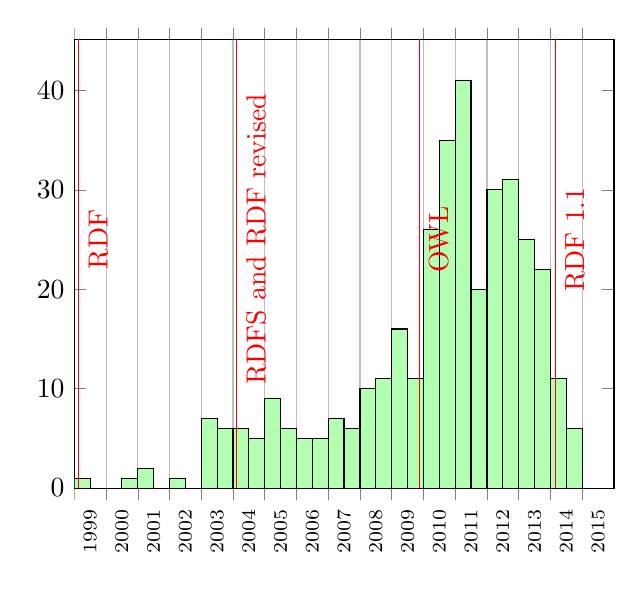
\begin{tikzpicture}
\begin{axis}[
date coordinates in=x,
x tick label style={align=left,rotate=90,font=\scriptsize},
date ZERO=1998-01-01,% <- improves precision!
xmin={1998-01-01}, % A date with no time is assumed to have a time of 00:00
xmax={2015-01-01},
ybar interval,
ymin={0},
  xticklabel={\year},
xtick={% Set tick marks CAREFUL the year has been decremented by one year ... was not able to figure out how to do that properly...
1998-01-01,
1999-01-01,
2000-01-01,
2001-01-01,
2002-01-01,
2003-01-01,
2004-01-01,
2005-01-01,
2006-01-01,
2007-01-01,
2008-01-01,
2009-01-01,
2010-01-01,
2011-01-01,
2012-01-01,
2013-01-01,
2014-01-01,
2015-01-01
},
]
\addplot[fill=green!30!white] coordinates {
(1998-01-01,1)
(1998-07-01,0)
(1999-01-01,0)
(1999-07-01,1)
(2000-01-01,2)
(2000-07-01,0)
(2001-01-01,1)
(2001-07-01,0)
(2002-01-01,7)
(2002-07-01,6)
(2003-01-01,6)
(2003-07-01,5)
(2004-01-01,9)
(2004-07-01,6)
(2005-01-01,5)
(2005-07-01,5)
(2006-01-01,7)
(2006-07-01,6)
(2007-01-01,10)
(2007-07-01,11)
(2008-01-01,16)
(2008-07-01,11)
(2009-01-01,26)
(2009-07-01,35)
(2010-01-01,41)
(2010-07-01,20)
(2011-01-01,30)
(2011-07-01,31)
(2012-01-01,25)
(2012-07-01,22)
(2013-01-01,11)
(2013-07-01,6)
(2014-01-01,0)
(2014-07-01,0)
};
\addplot[red,sharp plot,update limits=false] 
	coordinates {(1998-02-22,0) (1998-02-22,50)} 
	node[below, rotate=90] at (axis cs:1998-02-22,25) {RDF};
\addplot[red,sharp plot,update limits=false] 
	coordinates {(2013-02-25,0) (2013-02-25,50)} 
	node[below, rotate=90] at (axis cs:2013-02-25,25) {RDF 1.1};
\addplot[red,sharp plot,update limits=false] 
	coordinates {(2003-02-10,0) (2003-02-10,50)} 
	node[below, rotate=90] at (axis cs:2003-02-10,25) {RDFS and RDF revised};
\addplot[red,sharp plot,update limits=false] 
	coordinates {(2008-11-15,0) (2008-11-15,50)} 
	node[below, rotate=90] at (axis cs:2008-11-15,25) {OWL};
\end{axis}
\end{tikzpicture}
\caption{\label{fig:creaevol} Vocabularies distribution by creation date.}
\end{figure}

\begin{figure}[htb]
\makeatletter
\long\def\ifnodedefined#1#2#3{%
    \@ifundefined{pgf@sh@ns@#1}{#3}{#2}%
}
\makeatother

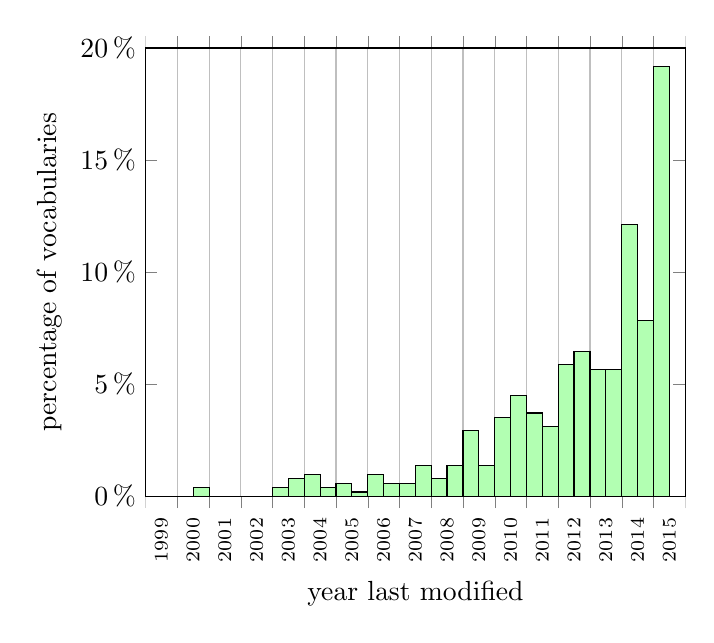
\begin{tikzpicture}
\begin{axis}[
    ylabel=percentage of vocabularies,
    xlabel=year last modified,
date coordinates in=x,
x tick label style={align=left,rotate=90,font=\scriptsize},
date ZERO=1998-01-01,% <- improves precision!
xmin={1998-01-01}, % A date with no time is assumed to have a time of 00:00
xmax={2015-01-01},
ybar interval,
ymin={0},
ymax={20},
yticklabel=\pgfmathprintnumber{\tick}\,$\%$,
  xticklabel={\year},
xtick={% Set tick marks CAREFUL the year has been decremented by one year ... was not able to figure out how to do that properly...
1998-01-01,
1999-01-01,
2000-01-01,
2001-01-01,
2002-01-01,
2003-01-01,
2004-01-01,
2005-01-01,
2006-01-01,
2007-01-01,
2008-01-01,
2009-01-01,
2010-01-01,
2011-01-01,
2012-01-01,
2013-01-01,
2014-01-01,
2015-01-01
},
]
\addplot[fill=green!30!white] coordinates {
(1998-01-01,0)
(1998-07-01,0)
(1999-01-01,0)
(1999-07-01,0.391)
(2000-01-01,0)
(2000-07-01,0)
(2001-01-01,0)
(2001-07-01,0)
(2002-01-01,0.391)
(2002-07-01,0.783)
(2003-01-01,0.978)
(2003-07-01,0.391)
(2004-01-01,0.587)
(2004-07-01,0.196)
(2005-01-01,0.978)
(2005-07-01,0.587)
(2006-01-01,0.587)
(2006-07-01,1.370)
(2007-01-01,0.783)
(2007-07-01,1.370)
(2008-01-01,2.935)
(2008-07-01,1.370)
(2009-01-01,3.523)
(2009-07-01,4.501)
(2010-01-01,3.718)
(2010-07-01,3.131)
(2011-01-01,5.871)
(2011-07-01,6.458)
(2012-01-01,5.675)
(2012-07-01,5.675)
(2013-01-01,12.133)
(2013-07-01,7.828)
(2014-01-01,19.178)
(2014-07-01,0)
};
\end{axis}
\end{tikzpicture}
\caption{\label{fig:modifevol} Vocabularies distribution by last modification date.}
\end{figure}

Looking at the creation date of the vocabularies registered in LOV, illustrated in Figure \ref{fig:creaevol}, it informs on the adoption of Semantic Web technologies. The apex of this bell curve is happening in 2011. The figure put as well this in the perspective of the W3C recommendation effort of RDF, RDFS and OWL languages. A decrease of vocabulary creation does not mean a decrease in use of the technology but rather than the coverage of existing vocabularies now covers a large part of the semantic description need. This is as well confirmed by figure \ref{fig:modifevol} that presents the last modification date of LOV vocabularies demonstrating a living ecosystem where vocabularies are not static. The median number of versions per vocabulary is 2. Where 98.23\% of vocabularies makes use of RDFS in addition to RDF, only 45.99\% of them makes use of OWL. 

Overall, LOV dataset contains almost 50,000 RDF vocabulary classes and properties with a median number of 9 and 17 respectively per vocabulary. Table \ref{tab:elements} presents a breakdown of LOV dataset content by vocabulary element type. Out of 511 vocabularies, 66.14\% use explicitly the English language for labels/comments. Table \ref{tab:language} presents the number and percentage of the top five languages detected in the LOV. Figure \ref{fig:langdist} shows the distribution of vocabularies per number of languages explicitly used: 27.98\% vocabularies still does not provide any language information and only 14.68\% of vocabularies are multilingual. 45 Languages are represented in LOV. We will discuss in section \ref{sec:conclusion} the importance for publishers to provide multilingual vocabularies on the Web.

\begin{table}[h!tb]
\caption{LOV vocabulary elements statistics.}
\begin{tabular}{lrr}
\hline
\textbf{Type} & \textbf{Count} &  \textbf{Median per vocab} \\ \hline
Classes & 20,034 & 9 \\
Properties & 29,925 & 17 \\
Instances & 5,232 & 0 \\
Datatypes & 101 & 0 \\
\hline  
\end{tabular}
\label{tab:elements}
\end{table}

 \begin{table}[h!tb]
\caption{Top five languages and percentage detected in the LOV catalogue. Some vocabularies can make use of multiple languages.}
\begin{tabular}{lrr}
\hline
\textbf{Language} & \textbf{Nb Vocabs} & \textbf{\% Vocabs (out of 511)}  \\ \hline
English & 338 & 66.14\%      \\
French & 37 & 7.24\%      \\
Spanish & 25 & 4.89\%      \\
German & 19 & 3.72\%      \\
Italian & 18 & 3.52\%      \\
\hline  
\end{tabular}
\label{tab:language}
\end{table}

\begin{figure}[htb]
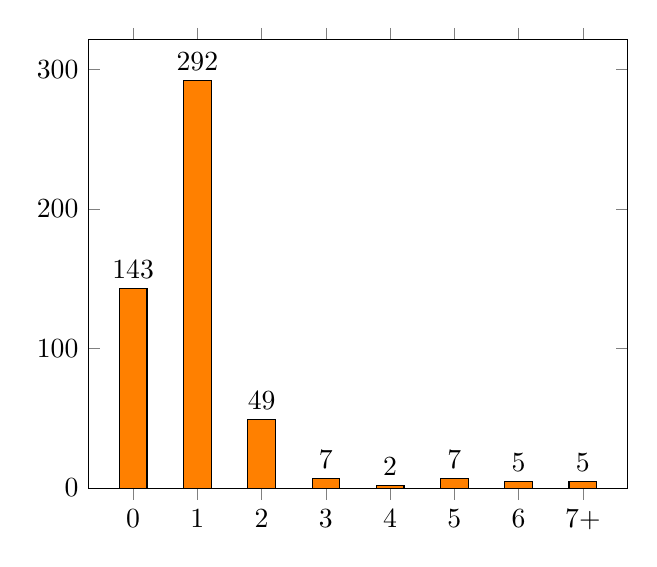
\begin{tikzpicture}
\begin{axis}[
    ybar,
    ymin={0},
    % ylabel={\#vocabularies},
    symbolic x coords={0,1,2,3,4,5,6,7+},
    xtick=data,
    nodes near coords,
    nodes near coords align={vertical},
    ]
\addplot[fill=orange] coordinates {(0,143)
(1,292)
(2,49)
(3,7)
(4,2)
(5,7)
(6,5)
(7+,5)
};
\end{axis}
\end{tikzpicture}
\caption{\label{fig:langdist} Distribution of the vocabularies per language count.}
\end{figure}

Over the last four years, the Linked Open Vocabularies initiative has gathered a community of around 470 people interested in various domains among them: ontology engineering or data publication. LOV Google+ community\footnote{\url{https://plus.google.com/communities/108509791366293651606}} is now an important place to discuss, report and announce general facts related to vocabularies on the Web. LOV dataset itself referenced 389 resources of type persons and 111 of type organization participating in vocabulary design and/or publication.



\section{System Components and Features}
	Figure \ref{fig:arch} shows an overview of the LOV components architecture. It is composed of four main components: 
\begin{inparaenum}[1)] 
	\item \emph{Tracking and Analysis}. Responsible to check for any vocabulary version update and analysing vocabularies specific features.
	\item \emph{Curation}. Ensure the high quality of the LOV dataset through methods for the community to suggest or edit the LOV catalogue.
	\item \emph{Data Access}. Consists in providing access to the data through a large range of methods and protocols to facilitate the use of LOV dataset and
	\item \emph{LOV User Interfaces and Application Program Interfaces}.
\end{inparaenum} 
Each components provides a set of features detailed in the following subsections.

The intended purpose of the LOV is to promote and facilitate the reuse of well documented vocabularies in the linked data ecosystem. To meet that goal, the LOV performs the following three main activities: 
\begin{inparaenum}[1)] 
  \item collecting new vocabularies from the LOV Community;
  \item tracking and analysis of the LOV vocabulary catalogue; and
  \item giving access to the data using various indices and publication methods to ease data consumption including a search engine, data dumps, SPARQL endpoint and APIs.
\end{inparaenum}
To carry out these tasks, the LOV is based on a number of components depicted in figure \ref{fig:arch}, relying on existing standards and open technologies.

\begin{figure}[ht!b]
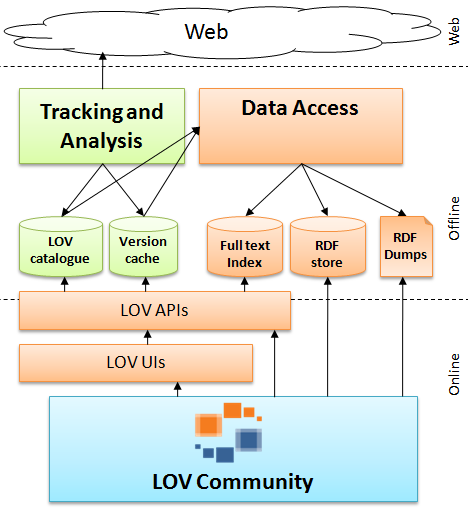
\includegraphics[scale=0.6]{lov_architecture.png}
\caption{Overview of the Linked Open Vocabularies Architecture.}
\label{fig:arch}
\end{figure}

\subsection{Tracking and Analysis}
	The \emph{Tracking and Analysis} component takes care of dereferencing\footnote{URI is looked up over HTTP to return content in a processable format such as XML/RDF, notation 3 or turtle.} LOV vocabularies. , storing a version locally (in notation 3 format) and extracting relevant metadata. A vocabulary consists of a collection of terms (classes and properties) expressed in W3C RDF, RDFS, OWL languages. 

At the Vocabulary level, the system extracts three types of information for each vocabulary version (figure \ref{fig:dcat}):
\begin{itemize}
\item Metadata associated to the vocabulary: this information is explicitly defined within the vocabulary to provide context, and useful data about the vocabulary. To be part of the LOV catalogue, a vocabulary must contain some minimal metadata information \cite{vandenbussche2011metadata}. Some high level vocabularies can be reused for that purpose, such as Dublin Core to describe authors, contributors, publishers or Creative Commons\footnote{\url{http://creativecommons.org/ns#}} for the description of a license.

\item Inlinks vocabularies, making explicit the \underline{links from} another vocabulary based on the semantic relation of their terms.

\item Outlinks vocabularies, making explicit the\\ \underline{links to} another vocabulary based on the semantic relation of their terms.
\end{itemize}

\subsubsection{Inter-vocabulary relationships} \label{voafRelations}
		There are many ways two vocabularies can rely on each other. Considering two vocabularies $V1$ and $V2$ such as $V1$ contains a class $c1$ and a property $p1$ and $V2$ contains a class $c2$ and a property $p2$. Relationships between these two vocabularies can be of the following types:
		\begin{description}
			\item [Import.] some terms from $V2$ are reused in complement with $V1$ to capture the semantic of the data:
\begin{lstlisting}[basicstyle=\tiny,float=htb,label=list:person, language=turtle]
<http://purl.org/NET/c4dm/event.owl> owl:imports 
	<http://www.w3.org/2006/time>
\end{lstlisting}
			\item [Specialization.] $V1$ defines some subclasses or subproperties (or local restrictions) of $V2$:
				\begin{itemize}
					\item c1 is subclass of c2 
\begin{lstlisting}[basicstyle=\tiny,float=htb,label=list:person, language=turtle]
<http://open.vocab.org/terms/Birth> rdfs:subClassOf 
	<http://purl.org/NET/c4dm/event.owl#Event>
\end{lstlisting}
					\item p1 is subproperty of p2.  
\begin{lstlisting}[basicstyle=\tiny,float=htb,label=list:person, language=turtle]
<http://purl.org/spar/fabio/hasEmbargoDate> 
	rdfs:subPropertyOf <http://purl.org/dc/terms/date>
\end{lstlisting}
				\end{itemize}

			\item [Generalization.] V1 defines some superclasses or superproperties of V2. c1 is superclass of c2 
\begin{lstlisting}[basicstyle=\tiny,float=htb,label=list:person, language=turtle]
<http://semanticweb.cs.vu.nl/2009/11/sem/Place> 
  skos:narrowMatch 
  <http://www.w3.org/2003/01/geo/wgs84_pos#SpatialThing>
\end{lstlisting}

			\item [Extension.] V1 extends the expressivity of V2:
				\begin{itemize}
					\item p1 is inverse of p2 
\begin{lstlisting}[basicstyle=\tiny,float=htb,label=list:person, language=turtle]
<http://vivoweb.org/ontology/core#translatorOf> owl:inverseOf
		<http://purl.org/ontology/bibo/translator>
\end{lstlisting}
					\item p1 has for domain c2.  
\begin{lstlisting}[basicstyle=\tiny,float=htb,label=list:person, language=turtle]
<http://xmlns.com/foaf/0.1/based_near> rdfs:domain
		<http://www.w3.org/2003/01/geo/wgs84_pos#SpatialThing>
\end{lstlisting}
				\end{itemize}

			\item [Equivalence.] V1 declares some equivalent classes or properties with V2.  
				\begin{itemize}
					\item p1 is equivalent to p2 
\begin{lstlisting}[basicstyle=\tiny,float=htb,label=list:person, language=turtle]
<http://lsdis.cs.uga.edu/projects/semdis/opus#journal_name> 
		owl:equivalentProperty 
		<http://purl.org/net/nknouf/ns/bibtex#hasJournal>
\end{lstlisting}
					\item c1 is equivalent to c2.  
\begin{lstlisting}[basicstyle=\tiny,float=htb,label=list:person, language=turtle]
<http://www.loc.gov/mads/rdf/v1#Language> owl:equivalentClass
		<http://purl.org/dc/terms/LinguisticSystem>
\end{lstlisting}
				\end{itemize}

			\item [Disjunction.] V1 declares some disjunct classes with V2. c1 is disjoint with c2 
\begin{lstlisting}[basicstyle=\tiny,float=htb,label=list:person, language=turtle]
<http://www.ontologydesignpatterns.org/ont/dul/DUL.owl#TimeInterval>
		owl:disjointWith 
		<http://www.ontologydesignpatterns.org/ont/dul/ontopic.owl#SubjectSpace>
\end{lstlisting}
		\end{description}

\begin{table}[h!tb]
\caption{Inter-vocabularies relationship types and their number of occurrences in LOV.}
\begin{tabular}{lcc}
\hline
\textbf{Inter vocabulary relationship} & \textbf{Nb Relations} \\ \hline
voaf:metadataVoc & 2637 \\
voaf:specializes & 1269 \\
voaf:extends & 1031 \\
owl:imports & 373 \\
voaf:hasEquivalencesWith & 201 \\
voaf:generalizes & 57 \\
voaf:hasDisjunctionsWith & 16 \\
\hline  
\end{tabular}
\label{tab:voaf}
\end{table}

\begin{figure}[ht!b]
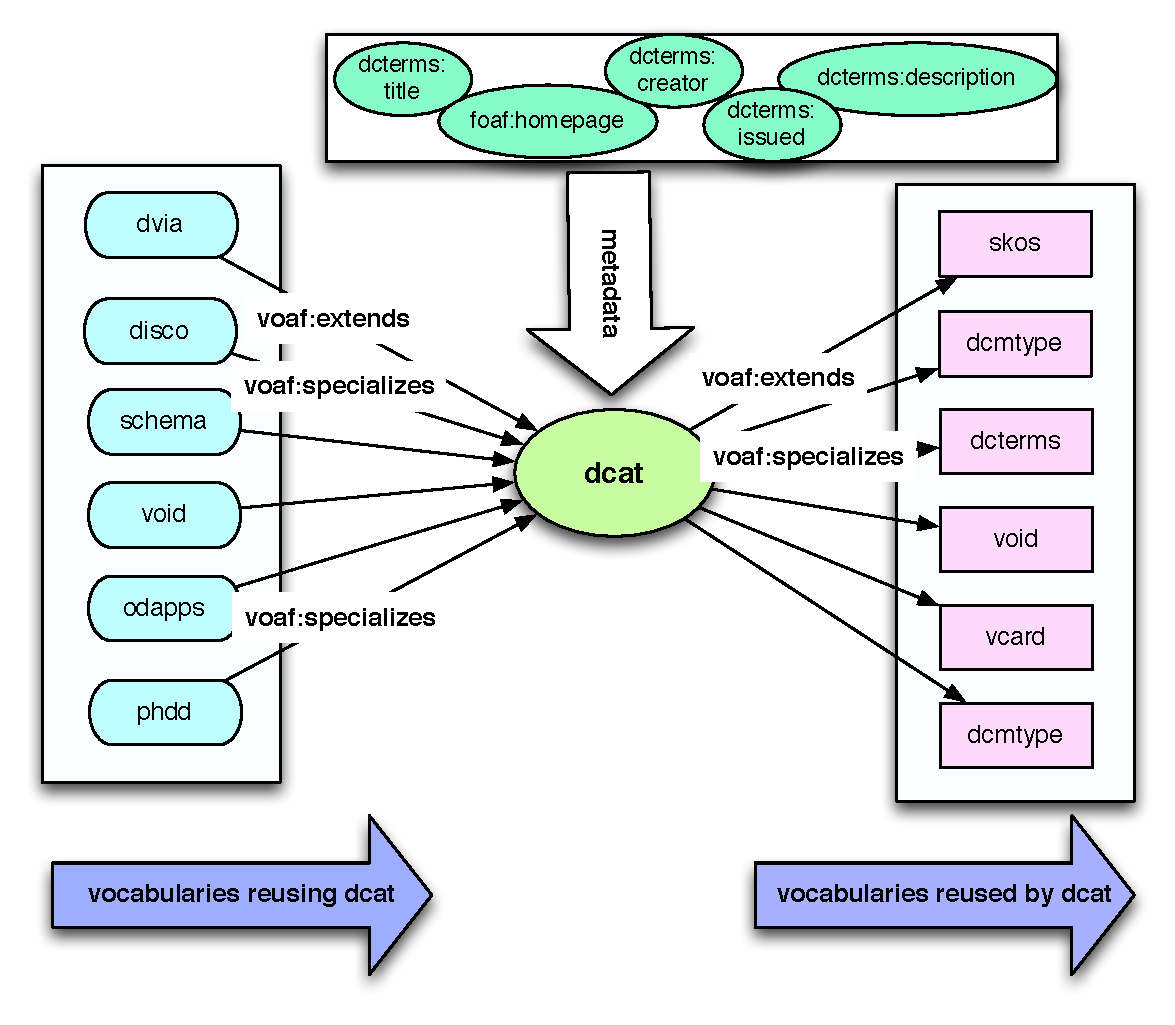
\includegraphics[scale=0.4]{dcat-relations.pdf}
\caption{Metadata type, vocabulary inlinks and outlinks of DCAT vocabulary.}
\label{fig:dcat}
\end{figure}

At the Vocabulary Term level, the system extracts labels that will be used for full text search and language information



\subsection{Curation}

The vocabulary collection is maintained by curators in charge of validating\footnote{Before a vocabulary is inserted, LOV curators contact the authors to make sure the vocabulary is published following the best practices and contains enough metadata}, inserting a vocabulary in the LOV ecosystem and assigning a detailed review (updated every year).

	\subsubsection{Vocabulary Insertion} Compared to other vocabulary catalogues (cf. section \ref{sec:related}), LOV relies on a semi-automated process for vocabulary insertion. Whereas an automated process put the emphasis on the volume, in our process, we focus on the quality of each vocabulary and therefore the quality of the overall LOV ecosystem. Suggestions are coming from the community and from inter-vocabulary reference links. Our system provides a feature to suggest\footnote{\url{http://lov.okfn.org/dataset/lov/suggest/}} the insertion of a new vocabulary. This feature allows a user to check what information the LOV application can automatically detect and extract. LOV curators then check if the vocabulary falls in the scope of LOV and if it meets basic vocabulary quality to be reused:
\begin{enumerate}
 \item a vocabulary should be dereferentiable
 \item a vocabulary should be parsable without error (warning tolerated)
 \item all classes and properties in a vocabulary should have an rdfs:label
 \item a vocabulary should refer and reuse relevant existing ones
\end{enumerate}
If a suggested vocabulary meets these criteria, it is then inserted in the LOV catalogue. during the process, the LOV curators keep the authors informed and help them to improve their vocabulary quality. As a result of our experience in vocabulary publication, we are now able to publish a handbook about Metadata recommendations for linked open data vocabularies to help that process~\cite{vandenbussche2011metadata}.

\begin{figure}[htb]
\tikzstyle{decision} = [diamond, draw, fill=blue!20, 
    text width=4.5em, text badly centered, node distance=3cm, inner sep=0pt]
\tikzstyle{block} = [rectangle, draw, fill=blue!20, text width=7em, text centered, minimum height=4em]
\tikzstyle{line} = [draw, -latex']
\tikzstyle{cloud} = [draw, ellipse,fill=red!20, node distance=3cm,
    minimum height=2em]
\tikzstyle{io} = [trapezium, trapezium left angle=70, trapezium right angle=110, draw, fill=blue!20,  text width=1em, text centered, minimum height=4em]

%\resizebox{!}{!}{%
\begin{tikzpicture}[node distance = 2cm, auto]
    % Place nodes
%   \node [block] (init) {initialize model};
%    \node [cloud, left of=init] (expert) {expert};
%    \node [io, right of=init, xshift=2cm] (system) {system};
%    \node [block, below of=init] (identify) {identify candidate models};
%    \node [block, below of=identify] (evaluate) {evaluate candidate models};
%    \node [block, left of=evaluate, node distance=3cm] (update) {update model};
%    \node [decision, below of=evaluate] (decide) {is best candidate better?};
%    \node [block, below of=decide, node distance=3cm] (stop) {stop};
%    % Draw edges
%    \path [line] (init) -- (identify);
%    \path [line] (identify) -- (evaluate);
%    \path [line] (evaluate) -- (decide);
%    \path [line] (decide) -| node [near start] {yes} (update);
%    \path [line] (update) |- (identify);
%    \path [line] (decide) -- node {no}(stop);
%    \path [line,dashed] (expert) -- (init);
%    \path [line,dashed] (system) -- (init);
%    \path [line,dashed] (system) |- (evaluate);

% Place nodes
\node [block] (authDesigns) {Author designs a vocabulary};
\node [block, below of=authDesigns] (authSuggest) {Author suggests a vocabulary};
\node [block, below of=authSuggest] (curFit) {Curator looks if the vocabulary is a good fit for LOV};
\node [block, left of=curFit] (botSuggest) {LOV Robot suggests a vocabulary};
\node [block, below of=botSuggest] (botDetects) {LOV Robot detects any reference to new vocabs in LOV ones};
\end{tikzpicture}
%}
\caption{\label{fig:creaevol} Vocabularies distribution by creation date.}
\end{figure}

\begin{figure}[ht!b]
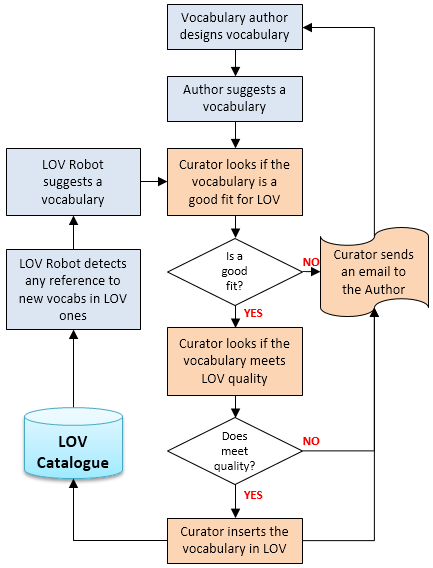
\includegraphics[scale=0.6]{workflow-curation-suggest.png}
\caption{Curation workflow for vocabulary insertion.}
\label{fig:arch}
\end{figure}

	\subsubsection{Vocabulary Review}
When some metadata failed to be extracted automatically (such as creators of a vocabulary), LOV curators enhance the description available in the system. The documentation provided by the LOV application assists any user in the task of understanding the semantics of each vocabulary term and therefore of any data using it. For instance, information about the creator and publisher is a key indication for a vocabulary user in case help or clarification is required from the author, or to assess the stability of that artifact. About 55\% of vocabularies specify at least one creator, contributor or editor. We augmented this information using manually gathered information, leading to the inclusion of data about the creator in over 85\% of vocabularies in the LOV. The database stores every version of a vocabulary since its first issue. For each version, a user can access the file (particularly useful when the original online file is no longer available). An automatic script is in place to automatically check for vocabulary updates on a daily basis. To embrace the complexity of the vocabulary ecosystem and assess the impact of a modification, one needs to know in which vocabularies and datasets a particular vocabulary term is referenced. For the first time LOV provides such a vision. 

\begin{figure}[ht!b]
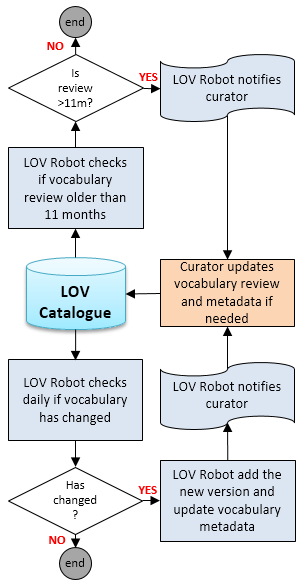
\includegraphics[scale=0.6]{workflow-curation-review.png}
\caption{Curation workflow for systematic vocabulary review.}
\label{fig:arch}
\end{figure}

\subsection{Data Access}

LOV system (code and data) is published under Creative Commons 4.0 license\footnote{\url{https://creativecommons.org/licenses/by/4.0/}} (CC BY 4.0). Four methods are offered for users and applications to access the LOV data:
		\begin{inparaenum}[1)] 
			\item query the LOV search engine to find the most relevant vocabulary terms, vocabularies or agents matching keywords;
			\item download data dumps of the LOV catalogue in RDF Notation 3 format or the LOV catalogue and the latest version of each vocabulary in RDF N-quads format;
			\item run SPARQL queries on the LOV SPARQL Endpoint; and
			\item use the LOV system Application Program Interface (API) which provides a full access to LOV data for software applications.
		\end{inparaenum}


\subsubsection{Search Engine}
For every vocabulary in the LOV, terms (classes, properties, datatypes, instances) are indexed and a full text search feature is offered\footnote{\url{http://lov.okfn.org/dataset/lov/terms}}. Compared to other existing ontology search engines (cf. section \ref{sec:related}), the Linked Open Vocabularies search engine ranking algorithm is not only based on term popularity in datasets but take as well into account its popularity within the LOV ecosystem and most importantly assigned a different score depending on which label property a searched term matched~\cite{butt2014}. We distinguish four different label property categories on which a search term could match: 
		\begin{itemize}
 			\item Local name (URI without the namespace). While a URI is not suppose to carry any meaning, it is a convention to use a compressed form of a term label to construct the local name. It becomes therefore an important artifact for term matching for which the highest score will be assigned. An example of local name matching the term ``person'' is \url{http://schema.org/Person};
			\item Primary labels. The highest score will also be assigned for matches on \url{rdfs:label}, \url{dce:title}, \url{dcterms:title}, \url{skos:prefLabel} properties. An example of primary label matching the term ``person'' is \url{rdfs:label} \emph{"Person"@en};
			\item Secondary labels. We define as secondary label the following properties: \url{rdfs:comment}, \url{dce:description}, \url{dcterms:description}, \url{skos:altLabel}. A medium score is assigned for matches on these properties. An example of secondary label matching the term ``person'' is \url{dcterms:description} \emph{"Examples of a Creator include a person, an organization, or a service."@en}; and
			\item Tertiary labels. Finally all properties not falling in the previous categories are considered as tertiary labels for which a low score is assigned. An example of tertiary label matching the term ``person'' is \url{http://metadataregistry.org/uri/profile/RegAp/name} \emph{"Person"@en}. 
		\end{itemize}
As a result a term matching a value for the property \url{rdfs:label} will have a higher score than if it matches a value for the property \url{dcterms:comment}. Based on the different nature of these labels, we apply different indexing tokenizers and scoring methods.

	\begin{table}[!htb]
		\caption{Two words, three words and more and URI search number in LOV.}
		\begin{tabular}{lcccc}
		\hline
		\textbf{Pattern} & \textbf{2012} & \textbf{2013} & \textbf{2014} & \textbf{Total} \\ \hline
		\textit{URI}  & 38   &  54  & 63  &  155      \\
		$t_{1}$ $t_{2}$ & 200 & 480 & 466 & 1146 \\
		($t_{1}$ $t_{2}$ $t_{3}$)* & 93 & 233 & 249 & 575\\
		\hline  
		
		\end{tabular}
		\label{tab:patterns}
	\end{table}

Human users or agents can further narrow a search by filtering on term type (class, property, datatype, instance), language, vocabulary domain and vocabulary. The LOV log of search terms between 2012-01-06 and 2014-12-09 presents a total of 54,657 terms, with 36,019 (65.90\%) duplicate terms and 18,643 unique terms (34.10\%). Figure \ref{fig:searchterms} depicts the number of terms in the log grouped by year. From 2012 to 2013, there has been an increase of more than 50\% of search in LOV. Searched terms are mostly single words (e.g., ``currency''). However, terms can be a composition of two words (e.g., ``family tree''), three words (e.g., ``semantic sensor network'') or an URI (e.g., ``http://www.aktors.org/ontology/portal''). Table \ref{tab:patterns} details the use of URIs, two words and at least three words for unique values in the LOV search log.
	
%	\begin{figure}[!htbp]
%	\centering{
%	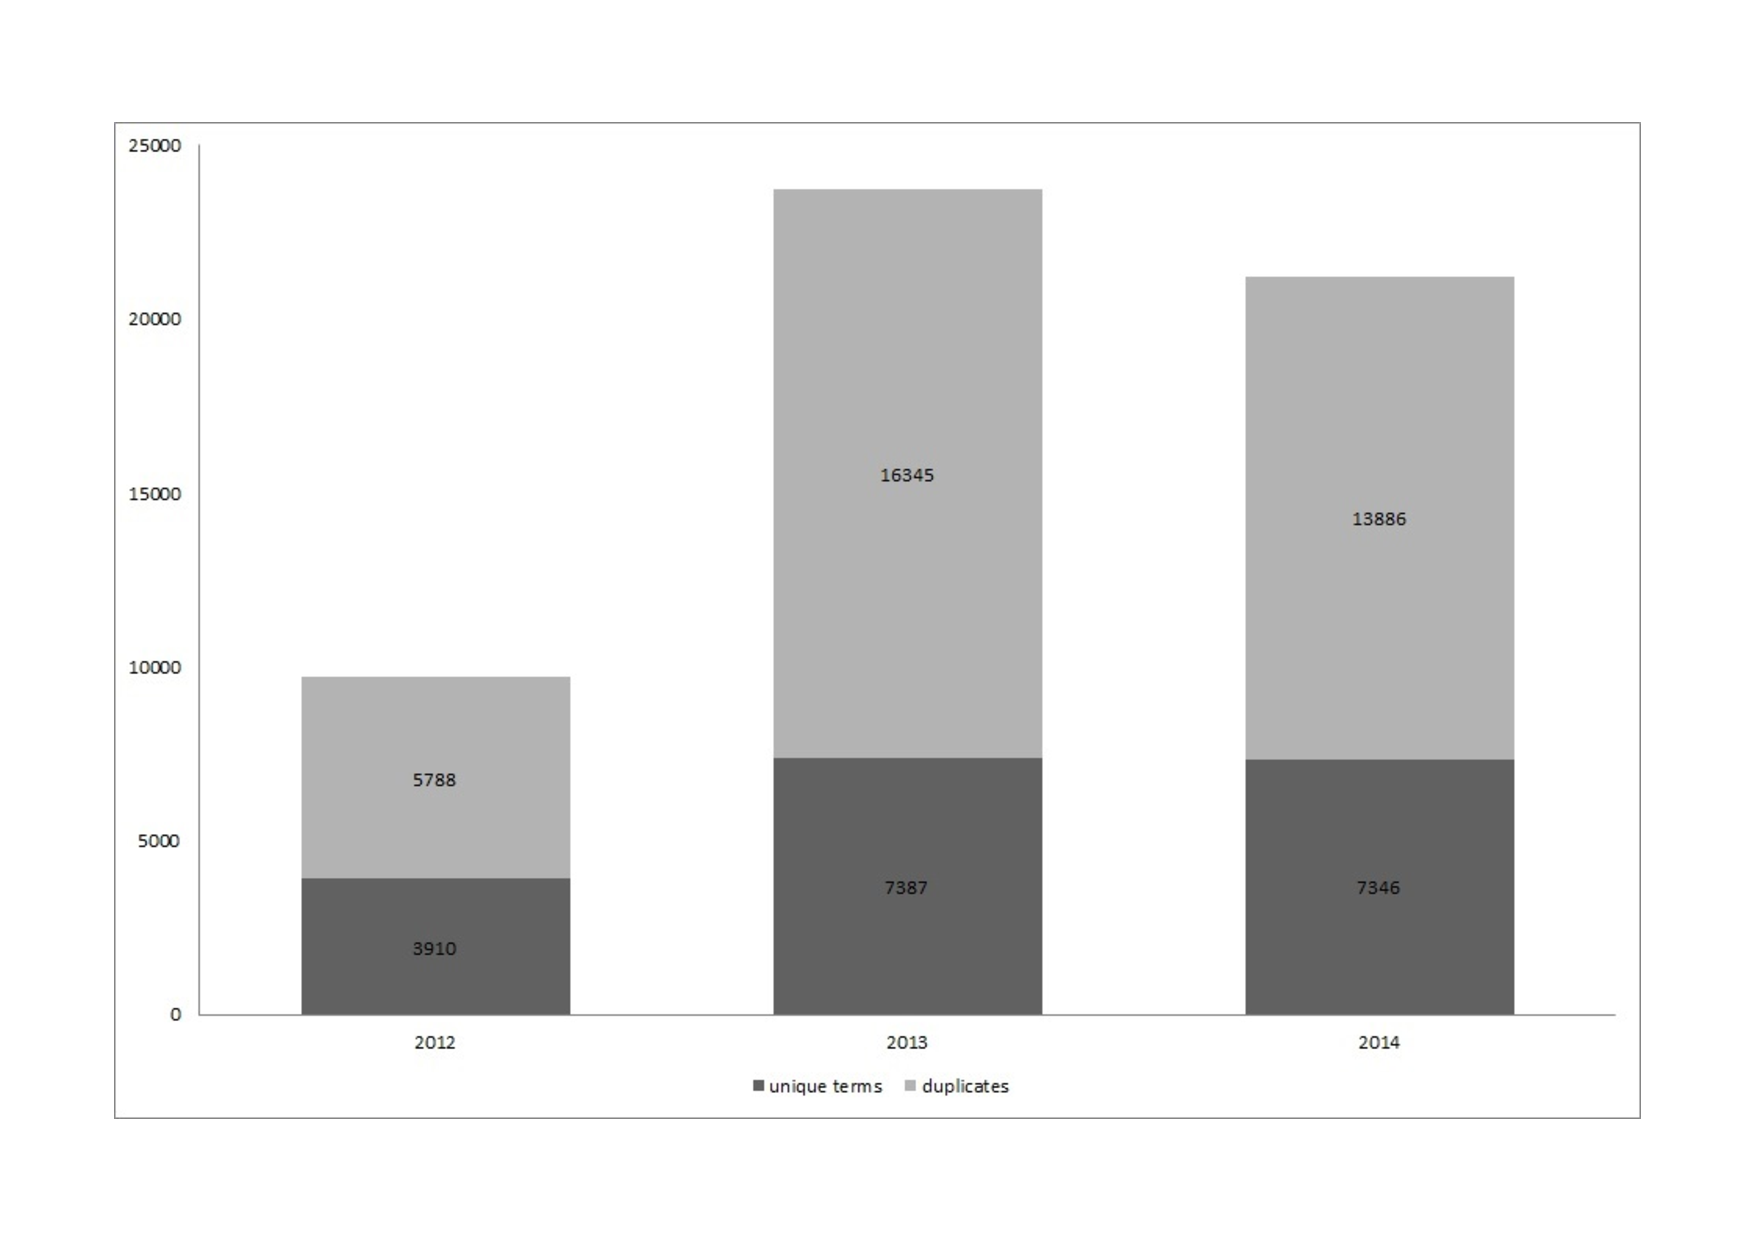
\includegraphics[scale=.28]{chart_searchterms.pdf}
%	\caption{Unique and duplicate terms searched by agents/users according to LOV log in the period between 2012/01/06 until 2014/12/09.}
%	\label{fig:searchterms}
%	}
%	\end{figure}

	\begin{figure}[tb]
	\ffigbox{
		\figfontsize%
		\begin{tikzpicture}
\begin{axis}[
legend style={at={(0.02,0.98)},anchor=north west,opacity=0.8, font=\scriptsize},
date coordinates in=x,
xticklabel={\year},
x tick label style={align=right,font=\scriptsize},
scaled ticks=false,
y tick label style={/pgf/number format/fixed},
date ZERO=2012-01-01, % Set near lowest date
xmin={2011-01-01}, 
xmax={2015-01-01},
ymin={0},
xtick={2012-01-01, % Set tick marks
2013-01-01,
2014-01-01},
grid=major,
point meta=explicit,
ybar stacked,
bar width=30pt,
every node near coord/.style={
        yshift=-15
    },
nodes near coords,
nodes near coords align=center
]


\pgfplotstableread{PGFPlots/LOVSearch.dat}\thisTable

\addplot+[black,fill=red] table[x=date,y=nbUnique, meta=nbUnique]{\thisTable};
\addlegendentry{Unique Terms}

\addplot+[black,fill=orange] table[x=date,y=nbDuplicates, meta=nbDuplicates]{\thisTable};
\addlegendentry{Duplicates}



\end{axis}
\end{tikzpicture}
	}{%
	  \caption{\label{fig:searchterms} Unique and duplicate terms searched by agents/users according to LOV log in the period between 2012-01-06 and 2014-12-09.}%
	}
	\end{figure}

\subsubsection{Data Dumps}
The system provides data dumps of the LOV vocabulary catalogue in RDF Notation 3 format\footnote{\url{http://lov.okfn.org/lov.n3.gz}} and the LOV catalogue along with the latest version of each vocabulary in RDF N-quads format\footnote{\url{http://lov.okfn.org/lov.nq.gz}}. As illustrated in figure \ref{fig:model}, the RDF model mainly reuses the Data CATalogue Vocabulary (DCAT) which allows the representation of the LOV catalogue as a \texttt{dcat:Catalog} composed of vocabulary entries (\texttt{dcat:CatalogRecord}) capturing information like the insertion date in LOV. Each entry point to the vocabulary itself is represented by a sub class of \texttt{dcat:Dataset} defined in the Vocabulary Of A Friend (VOAF). This artifact contains metadata extracted by LOV application such as creators, first issued date, number of occurrences of the vocabulary in Linked Open Data. Each vocabulary is then linked to its various published versions represented by the \texttt{dcat:Distribution} entity on which information such as inter vocabulary links or languages can be found.

\begin{figure*}[!htb]
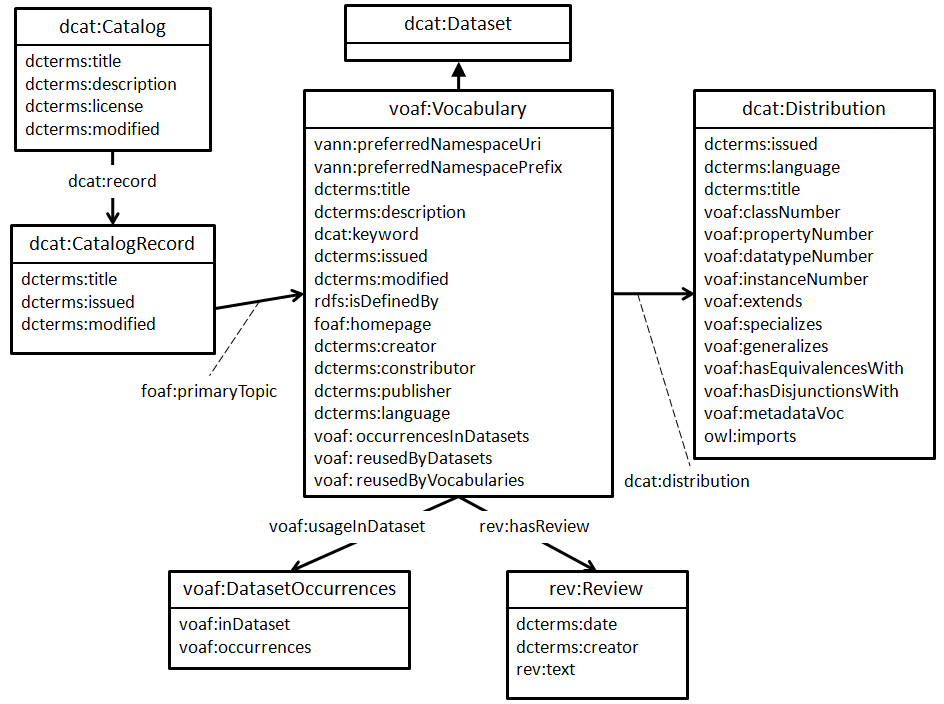
\includegraphics[scale=0.5]{model.png}
\caption{UML class diagram representation of LOV catalogue RDF schema model.}
\label{fig:model}
\end{figure*}


\subsubsection{SPARQL Endpoint}
The LOV SPARQL Endpoint\footnote{\url{http://lov.okfn.org/dataset/lov/sparql}} offers a complementary data access method and allows clients to pose complex queries to the server and retrieve direct answers computed over the LOV dataset. We use Jena fuseki triple store to store the N-quads file containing the LOV catalogue and the latest version of each vocabulary. This allows for the first time to query multiple vocabulary at the same time and to detect inter-vocabulary dependencies. An example of this use is explained in section \ref{sec:dataPubOntoEngine}.

\subsection{LOV User Interfaces and Application Program Interfaces}
LOV APIs give a remote access to the many functions of LOV through a set of RESTful services\footnote{\url{http://lov.okfn.org/dataset/lov/apidoc/}}. The basic design requirements for these APIs is that they should allow applications to get access to the very same information humans do via the User Interfaces. More precisely the APIs give access, through three different type of services (cf. figure \ref{fig:apis}), to functions related to:
\begin{itemize} 
			\item Vocabulary terms (classes, properties, datatypes and instances). With these functions, a software application can query the LOV search engine, ask for autocompletion or suggestion for misspelled terms;
			\item Vocabularies. A client can get access to the current list of vocabularies contained in the LOV catalogue; search for vocabularies, get autocompletion or obtain all details about a vocabulary; and
			\item Agents. This provides a software agent with a list of all agents references in the LOV catalogue, a mean to search for an agent, get autocompletion and details about an agent.
		\end{itemize}
LOV APIs is a convenient manner to get access to the full functionality and data of the LOV. It is particularly appropriate for dynamic Web applications using scripting languages such as Javascript. The APIs described above have been developed for, and following the requirements of, Ontology Design and Data Publication tools.

\begin{figure}[ht!b]
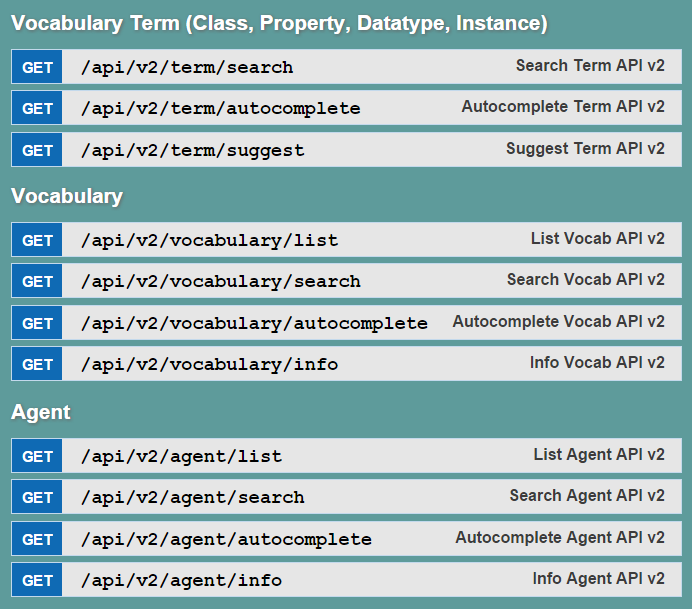
\includegraphics[scale=0.4]{apis.png}
\caption{List of APIs to access LOV data.}
\label{fig:apis}
\end{figure}

The LOV Website offers an intuitive navigation within the vocabularies catalogue. It allows users to explore vocabularies, vocabulary terms, agents, languages and to get the connection between these entities. For instance, a user can look for experts in \emph{geography} and \emph{geometry} domains\footnote{\url{http://lov.okfn.org/dataset/lov/agents?&tag=Geography,Geometry}}. We use d3\footnote{\url{http://d3js.org/}} javascript library to display charts and make the navigation more interactive like star graph representation used to display incoming and outgoing links between vocabularies (cf. figure \ref{fig:graphVocab}). 


\begin{figure}[ht!b]
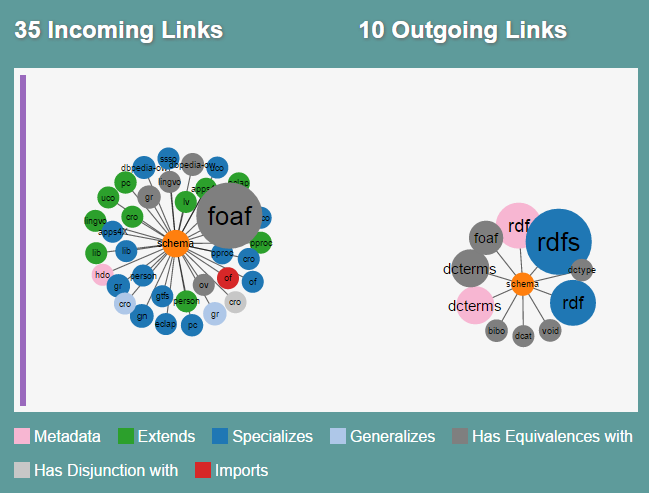
\includegraphics[scale=0.45]{graphVocab.png}
\caption{Schema.org vocabulary incoming and outgoing links graphical representation as displayed in the UI.}
\label{fig:graphVocab}
\end{figure}




\section{LOV as a support for Data Publication and Ontology Engineering}
\label{sec:dataPubOntoEngine}


LOV can be used in any methodology for the creation and reuse of ontologies. One of the most mature methodology for supporting collaborative development of ontologies is NeOn.  
The NeOn Methodology is a scenario-based methodology that supports the collaborative aspects of ontology development and reuse, as well as the dynamic evolution of ontology networks in distributed environments \cite{MC10}. 
%The key assets of the NeOn Methodology are \cite{MC10}:
%\begin{itemize}
% \item  A set of nine scenarios for building ontologies and ontology networks, emphasizing the reuse of ontological and non-ontological %resources, the re-engineering and merging, and taking into account collaboration and dynamism.
% \item The NeOn Glossary of Processes and Activities, which identifies and defines the processes and activities carried out when ontology %networks are collaboratively built by teams.
% \item Methodological guidelines for different processes and activities of the ontology network development process, such as the reuse and re-%engineering of ontological and non-ontological resources, the ontology requirements specification, the ontology localization, the scheduling, %etc.
%\end{itemize}

Based on the NeOn Methodology's glossary of activities for building ontologies, the LOV system is relevant in four activities:

\begin{description}

 \item [Ontology Search.] Main LOV's feature is the search of vocabulary terms. These vocabularies are categorized within the LOV according to the domain they address. In this way, the LOV system contributes to ontology search by means of (a) keyword search and (b) domain browsing.
 \item [Ontology Assessment.] LOV provides a score for each term retrieved by a keyword search. This score can be used during the assessment stage.
 \item [Ontology Mapping.] In LOV, vocabularies rely on each other in seven different ways. These relationships are explicitly stated using VOAF vocabulary\footnote{\url{http://purl.org/vocommons/voaf}}. This data could be useful to find alignments between ontologies, for example one user might be interested in finding equivalent classes for a given class or all the equivalent classes among two ontologies. Listing \ref{list:alignment} shows the SPARQL query to retrieve all the equivalent classes and properties between the vocabularies \texttt{foaf} and \texttt{dcterms}\footnote{The reader can run the query on LOV Endpoint: \url{http://goo.gl/sTIGQ6}. Prefixes are omitted for readability purpose. They can be found in LOV.}.
     
 \begin{lstlisting}[basicstyle=\tiny,float=htb,caption={SPARQL query asking for all the equivalent classes and properties between the vocabularies foaf and dcterms. },label=list:alignment, language=turtle]
 PREFIX owl:<http://www.w3.org/2002/07/owl#>
 SELECT DISTINCT ?elem1 ?alignment ?elem2 {
   {?elem1 owl:equivalentClass ?elem2}
      UNION {?elem1 owl:equivalentProperty ?elem2}
      UNION {?elem2 owl:equivalentClass ?elem1}
      UNION {?elem2 owl:equivalentProperty ?elem1}
      FILTER(!isBlank(?elem2))
      FILTER(!isBlank(?elem1))
      ?elem1 ?alignment ?elem2.
      ?elem1 rdfs:isDefinedBy 
		<http://xmlns.com/foaf/0.1/>.
      ?elem2 rdfs:isDefinedBy 
		<http://purl.org/dc/terms/>.
 } ORDER BY ?alignment
	
	\end{lstlisting}
	
	Figure \ref{fig:eqCR} shows the alignments between foaf and dcterms vocabularies by mean of \url{owl:equivalentClass} and \\ \url{owl:equivalentProperty}.
    \begin{figure}
      \centering
      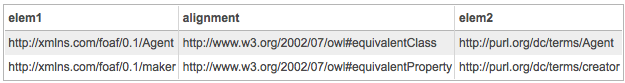
\includegraphics[width=1.0\linewidth]{equivalentCandR.png}
      \caption{Equivalent classes and properties between foaf and dcterms}
      \label{fig:eqCR}
    \end{figure}
    
% \item [Ontology Localization.] Labels in different languages are stored in the LOV endpoint. This annotations could be used when translating terms into different languages. This information could be extracted by querying the SPARQL endpoint\footnote{Result of the query can be found at the following URL: \url{http://goo.gl/JJCJ01}} as shown in Listing \ref{list:person} where all the labels defined for the terms that have at least one \url{rdfs:label} containing strictly ``person":
		
%    \begin{lstlisting}[basicstyle=\tiny,float=htb,caption={SPARQL query asking all the labels defined for the terms containing person.},label=list:person, language=turtle]
% SELECT DISTINCT ?label2 ?element{
%   ?element rdfs:label ?label1 .
%   ?element rdfs:label ?label2 .
%   FILTER (?label1 != ?label2 ).
%   FILTER(REGEX(STR(?label1), "person", "i")).
% } ORDER BY ?element
%	\end{lstlisting}
%							
%   An excerpt of the query result is shown in Figure \ref{fig:translations}. From that result, ``Persona''@es and ``Personne''@fr could be used as translations for the English term ``Person'' in Spanish and French respectively. 
%   
%   \begin{figure}[ht!b]
%     \centering
%     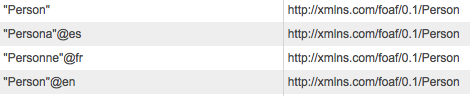
\includegraphics[width=.90\linewidth]{translations1.png}
%     \caption{Translations example for foaf:Person}
%     \label{fig:translations}
%   \end{figure}
   
\end{description}

Figure \ref{fig:LOVandNeOn} shows the activities within the overall NeOn methodologies activity workflow that can benefit from the LOV.
\begin{figure}[h!tp]
\centering
  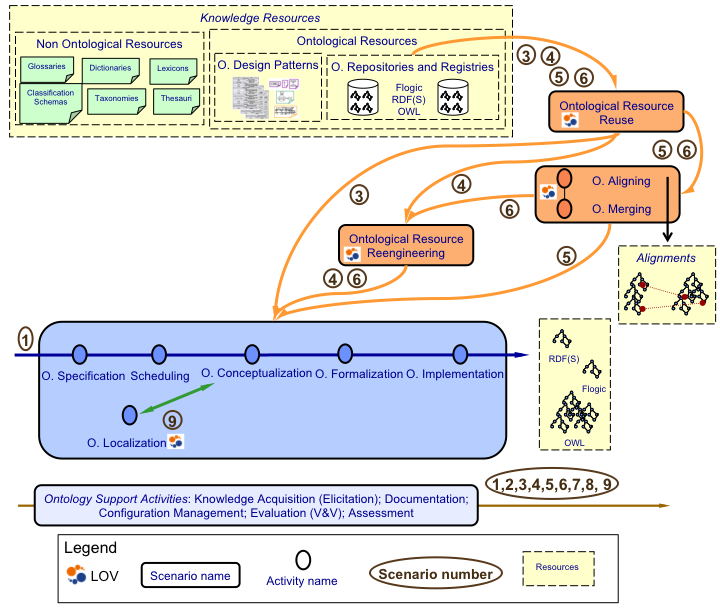
\includegraphics[width=1\linewidth]{neonScenarios.png}
  \caption{Meeting points between the LOV and the NeOn methodology, derived from \cite{MC10}.}
  \label{fig:LOVandNeOn}
\end{figure}

\section{LOV Adoption}
\label{sec:lovecosystem}
The LOV is supporting the emergence of a rich application ecosystem thanks to its various data access methods. We list below some tools using our system as part of their service and projects using LOV as a research artifact.
 
\subsection{Derived tools and applications}

Maguire et al. \cite{ontomaton12} uses the LOV search API to implement OntoMaton\footnote{\url{https://github.com/ISA-tools/OntoMaton}}, a widget for bringing together ontology lookup and tagging within the collaborative environment provided by Google spreadsheets. 

YASGUI (Yet Another SPARQL Query GUI)\footnote{\url{http://yasgui.laurensrietveld.nl}} is a client-side JavaScript SPARQL query editor that uses the LOV API for property and class autocompletion together with \url{http://prefix.cc} for namespace prefix autocompletion \cite{yasgui}.

Datalift\footnote{\url{http://datalift.org/en/node/24}} platform \cite{scharffe_2012}, a framework for ``lifting'' raw data into RDF, comes with a module to map data objects and properties to ontology classes and predicates available in the LOV catalogue. Data2Ontology module takes as input a ``raw RDF'', that is a dataset that has been converted directly from legacy format to triples. The goal is to help publishers reuse existing ontologies for converting their dataset owing easy discovery and interlinking. 
%It consists of three main components assisting the publisher in selecting properties suitable for the dataset to be published. 
%\begin{description}
%\item 1-LOV component. This component connects with the LOV catalogue to retrieve up-to-date ontologies using the LOV %search API\footnote{\url{http://lov.okfn.org/dataset/lov/apidoc/#lov2search}}.
%\item 2-Matching Workflow. Data2Ontology maps the data to LOV by automatically proposing a list of best matches.
%\item 3-SPARQL Generator. This module receives as input the desired mappings and creates the SPARQL CONSTRUCT query needed to %implement the mapping. The query can further be modified before the execution to generate a new dataset in the lifting process with Datalift.
%\end{description}

OntoWiki\footnote{\url{http://ontowiki.net/}} facilitates the visual presentation of a knowledge base as an information map, with different views on instance data \cite{auer2006ontowiki}. It enables intuitive authoring of semantic content, with an inline editing mode for editing RDF content, similar to WYSIWIG for text documents. OntoWiki offers a vocabulary selection feature based on LOV.

%Prot{\'e}g{\'e}LOV\footnote{\url{http://labs.mondeca.com/protolov/} provides a technological support to help users in reusing terms based on the LOV API. It is a plug-in in Prot{\'e}g{\'e} [cite] for easing the development of ontologies by reusing existing vocabularies at low fine grained level. The tool helps to improve the modeling and reuse of ontologies used in the LOD cloud. 

\subsection{Using LOV as a Research platform}

The LOV has served as the object of studies in \cite{poveda2012landscape} where Poveda-Villal\'on \emph{et al.} analysed trends in ontology reuse methods. In addition, the LOV dataset has been used in order to analyze the occurrence of good and bad practices in vocabularies \cite{poveda2013detecting}.

Prefixes in the LOV dataset are regularly mapped with namespaces in the prefix.cc service. In \cite{wasabi13}, the authors perform alignments of Qnames of vocabularies in both services, and provide different solutions to handle clashes and disagreements between preferred namespaces. Both the LOV and prefix.cc provide associations between prefixes and namespaces but follow a different logic. The prefix.cc service supports polysemy and synonymy, and has a very loose control on its crowd-sourced information. In contrast, the LOV has a much more strict policy forbidding polysemy and synonymy ensuring that each vocabulary in the LOV database is uniquely identified by a unique prefix identification allowing the usage of prefixes in various LOV publication URIs. This requirement leads sometimes to a situation where the LOV use prefixes differently from the ones recommended by the vocabulary publishers.

The LOV query log covering the period between 2012-01-06 and 2014-04-16 is used in \cite{butt2014} to build a benchmark suite for ontology search and ranking. The CBRBench\footnote{\url{https://zenodo.org/record/11121}} benchmark uses eight ranking models of resources in ontologies and compares the results with ontology engineers. We plan to start a collaboration with the authors to enhance the LOV search based on the study result.

In \cite{janowicz2014five}, the authors rate vocabularies according to some criteria beyond the sameAs links but subClassOf and equivalentClass 'links' between vocabularies to foster interoperability, query federation, ease the interpretation of data, and so forth. %\ghis{ read this paper to add more content here}

RDFUnit\footnote{\url{https://github.com/AKSW/RDFUnit}} is a test-driven data debugging framework for the Web of Data. In \cite{rdfunit}, the authors provide an automatic test case for all available schema registered with the LOV. Vocabularies are used to encode semantics to domain specific knowledge to check the quality of data.

Governatori et al. \cite{governatori2014} analyzes the current use of licenses in vocabularies on the Web based on the LOV catalogue to further propose a framework to detect incompatibilities between datasets and vocabularies.


\section{Related work}
\label{sec:related}

Reusing vocabularies requires searching for terms in existing specialized vocabulary catalogues or search engines on the web. While we refer the reader to~\cite{AquinJoWS12} for a systematic survey of ontology repositories, we list below some existing catalogues relevant to find vocabularies:
\begin{itemize}
 \item \textit{Catalogues of generic vocabularies/schemas} similar to LOV catalogue. Example of catalogues falling in this category are vocab.org\footnote{\url{http://vocab.org/}}, ontologi.es\footnote{\url{http://ontologi.es/}}, JoinUp Semantic Assets or the Open Metadata Registry.
 \item \textit{Catalogues of ontologies for a specific domain} such as biomedicine with the BioPortal \cite{bioportal11}, geospatial ontologies with SOCoP+OOR\footnote{\url{http://socop.oor.net/}}, Marine Metadata Interoperability and the SWEET \cite{sweet05} ontologies\footnote{\url{http://sweet.jpl.nasa.gov/2.1/}}. The SWEET ontologies include several thousand terms, spanning a broad extent of Earth system science and related concepts (such as data characteristics), with the search tool to aid finding science data resources. 
 \item \textit{Catalogues of ontology Design Patterns (ODP)} focused on reusable patterns in ontology engineering \cite{presutti08}. The submitted patterns are small pieces of vocabularies that can further be integrated or linked with other vocabularies. ODP does not provide a search function for specific terms as is the case with Swoogle or Watson.
 \item \textit{Search Engines of ontology terms}. Among ontology search engines, we can cite: Swoogle \cite{finin2005swoogle}, Watson \cite{d2007watson,Sabou07} and FalconS \cite{cheng2008falcons}. These search engines crawl for data schema from RDF documents on the Web. They offer a filtering based on ontology type (Class, Property) and a ranking based on the popularity. They don't look for ontology relations nor check if the definition of the ontology is available (usually known as dereferenciation)
\end{itemize}


The LOV focuses only on vocabularies (subpart of semantic documents of the web) submitted by the community, reviewed and validated by curators. In addition, the LOV keeps track locally of all versions of the vocabularies.  In contrast, Swoogle is designed to automatically discover Semantic Web Documents (SWDs), index their metadata. Thus, the result of a search query retrieved any semantic document. For example, a query of the term \textit{person} gives $16,438$ results while in the LOV, the term only appears in $1,562$ vocabularies.
Watson works similarly to Swoogle, crawling and indexing semantic documents at a small scale, explicitly distinguishing for each document (resource), concepts, properties and individuals if available. While in Swoogle  the ranking score is displayed, Watson shows the language of the resource and the size. Falcons is a keyword-based search system for concepts and objects on the Semantic Web, and is equipped with entity summarization for browsing. It is notable that Falcons limits the search only to ontologies and a recommendation feature is provided according to users' preferences. However, it does not provide any relationships between the related ontologies, nor any domain classification of the vocabularies.
Table \ref{tab:lovfeatures} compares key features of LOV with respect to Swoogle, Watson and Falcons.
 \begin{table*}[!htb]
\centering{
\begin{tabular}{lllll}
\hline
 \textbf{Feature}	& Swoogle & Watson & Falcons & LOV 			 \\ \hline
Browsing ontologies	   & Yes & Yes & Yes & Yes \\
Ontology Discovery Method   & Automatic & Automatic & Automatic & Manual \\
Scope & SWDs & SWDs & Concepts & Ontologies \\
Ranking	& LOD popularity & LOD popularity & LOD popularity &  LOD/LOV popularity\\
&&&&+ property semantic score	 \\
Domain filtering & No & No & No & Yes \\
Comments and review 	& No & Yes & No & Only by curators	\\
Web service access & Yes & Yes & Yes & Yes		\\
SPARQL endpoint	& No & No & No & Yes		\\
Read/Write	& Read & Read \& Write & Read &Read  	\\
Ontology directory & No & No & No &Yes \\
Application platform & No & No & No & Yes \\
Storage & Cache & - & - & Dump \& endpoint \\
Interaction with Contributors & No &  - & No & Yes \\

		\\ \hline

\end{tabular}
\caption{Comparison of LOV, with respect to Swoogle, Watson and Falcons; based on part of the framework defined in \cite{AquinJoWS12}.  }
\label{tab:lovfeatures}
}
\end{table*}


\section{Discussion}

Apart form the core features for ontology development as search, ranking and reuse, LOV provides aside useful functionalities  for ontology development processes and activities. For example, one could take advantage of LOV to localize ontologies or provide multilingual annotation as rdfs labels in different languages are stored in the LOV endpoint. This annotations could be used when translating terms into different languages or to provide multilingual search based on ontologies. 
		
%    \begin{lstlisting}[basicstyle=\tiny,float=htb,caption={SPARQL query asking all the labels defined for the terms containing person.},label=list:person, language=turtle]
% SELECT DISTINCT ?label2 ?element{
%   ?element rdfs:label ?label1 .
%   ?element rdfs:label ?label2 .
%   FILTER (?label1 != ?label2 ).
%   FILTER(REGEX(STR(?label1), "person", "i")).
% } ORDER BY ?element
%	\end{lstlisting}
%							
%   An excerpt of the query result is shown in Figure \ref{fig:translations}. From that result, ``Persona''@es and ``Personne''@fr could be used as translations for the English term ``Person'' in Spanish and French respectively. 
%   
%   \begin{figure}[ht!b]
%     \centering
%     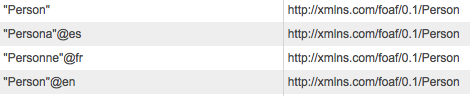
\includegraphics[width=.90\linewidth]{translations1.png}
%     \caption{Translations example for foaf:Person}
%     \label{fig:translations}
%   \end{figure}

%The LOV search engine is to the best of our knowledge, the only purpose-built ontology search engine available on the Web with an up-to-date index.

\section{Conclusion and Future work}
\label{sec:conclusion}
In this system report, we presented an overview of the Linked Open Vocabularies initiative. The importance of this work is motivated by the difficulty for data publishers to determine which vocabularies to use to describe their data. The key innovations described in this article include: 
\begin{inparaenum}[1)] 
	\item the availability of a high quality vocabularies dataset through multiple accessing methods;
	\item the vocabulary metadata curation by experts, making explicit for the first time the relationships between vocabularies and their version history; and
	\item the consideration of property semantic in term search scoring.
\end{inparaenum}

The adoption and integration of the LOV catalogue in applications for vocabulary engineering, reuse and data quality are significant. Linked Open Vocabularies have a central role in vocabulary life-cycle on the Web of Data as highlighted by the W3C\footnote{\url{http://www.w3.org/2013/data/}}. In the future, we see in particular the following directions for advancing the LOV initiative:

\emph{From single to multi-term search.} An area which is still largely unexplored is multi-term vocabulary search. During the ontology design process, it is common to have more than 20 concepts to be represented using existing vocabularies or a new one in case there is no corresponding artifact. While we are able to search for relevant terms in the LOV it is still the responsibility of the ontology designer to understand the complex relationships betwen all these terms and come up with a coherent ontology. We could use the network of vocabularies defined in the LOV to suggest not only a list of terms but graphs to represent several concepts together.

\emph{Multilingual vocabularies.} There is a need for vocabularies to support more languages. Labels are the main entrypoint to a vocabulary and their associated language is the key. Only 18\% of LOV vocabularies use a different language than English. Multilingualism is important at least for two reasons: 
\begin{inparaenum}[1)] 
	\item the most obvious one is allowing users to search, query and navigate vocabularies in their native language; and
	\item translating is a process through which the quality of a vocabulary can only improve. Looking at a vocabulary through the eyes of other languages and identifying the difficulties of translation helps to better outline the initial concepts and if necessary refine or revise them. 
\end{inparaenum} 
Hence multilingualism and translation should be native, built-in features of any vocabulary construction, not a marginal task.

\emph{Query extension and rewriting.} Another research perspective is SPARQL query extension and rewriting based on Linked Vocabularies. Using the inter-vocabulary relationships we could transform the query to use the same semantic (same vocabulary terms) as the data source(s) to query.

\section*{Acknowledgments}
This work has been partially supported by the French National Research Agency (ANR) within the Datalift Project, under grant number ANR-10-CORD-009; the Spanish project BabelData (TIN2010-17550) and Fujitsu Laboratories Limited. The Linked Open Vocabularies initiative is graciously hosted by the Open Knowledge Foundation. We would like to thank all the members of the LOV community, all the editors and publishers of vocabularies who trust in the LOV catalogue. 


\bibliographystyle{plain}
\bibliography{lov}
\end{document}
